%\section{ Hamiltonian theory}
%\label{sec:theory}
The Hamiltonian for resonant electrons in the frame of reference moving with the local resonance is obtained through canonical transformation \cite{zheng2024}. We analyze the wave-particle interaction on discrete local spatial cells, with phase space characterized by new canonical coordinates $(\xi$, $\Omega)$. In the original Hamiltonian, $\xi$, $\Omega$ phase space is decoupled for each cell at position $s_i$ along the magnetic field. In our hybrid Vlasov simulation \cite{zheng2023b,zheng2024}, we separately examine the phase flow for the onset of chorus using the following Hamiltonian,
\begin{equation}\label{eq.H_lab}
    K = \frac{k_l^2\Omega^2}{2} + \mathbb{R}\left(\frac{\omega_b^2}{k_l^2} (e^{-\imath \xi} + \alpha \cdot \xi) \right)~,
\end{equation}
where $\mathbb{R}$ denotes taking the real part.
The inhomogeneous parameter $\alpha$ satisfies
\begin{equation}\label{eq.alpold}
   \alpha  = \frac{k_l}{\omega_b^2}(\mathcal{J} - \frac{\Pi}{2}) \frac{d\omega_{ce}}{ds}~,
\end{equation}
and the bounce frequency satisfies
\begin{equation}
    \frac{\omega_b^2}{k_l^2} = \sqrt{2\omega_{ce}\mu}a(s_i,t)~,
\end{equation}
where $\mu = \mathcal{J}+\Pi+\Omega$. 
Note that $\mathcal{J}$ is another canonical momentum associated with the slow scale motion along field line. Gyro frequency $\omega_{ce}$, and parameter $\Pi = (\omega - \omega_{ce})/k^2$ are determined from background plasma parameter on each local cell \cite{zheng2024,zheng2023b}. The background magnetic field and $\Pi$ parameters are shown in Figs. \ref{fig.aanda}(a) and (b).

\begin{figure}
    \centering
    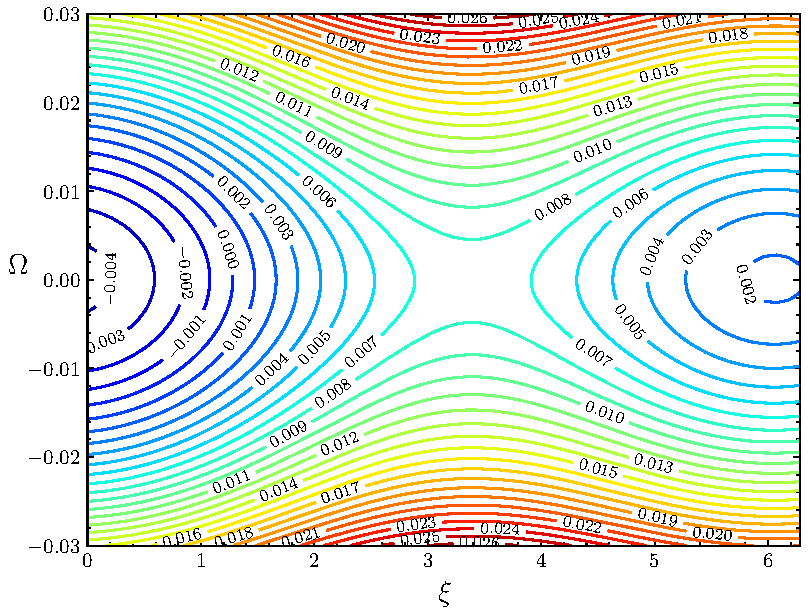
\includegraphics[scale=0.5]{img/Hamcontour.pdf}
    \caption{The contour plot of Hamiltonian in Eq. (\ref{eq.H_lab}) (a) and  Eq. (\ref{eq.H_frame}) (b) using fixed $\mathcal{J}, a, \Pi$ parameters. The dots and red cross denotes the initial location for the test particle tracing.
    \label{fig.Hamcontour}
    }
\end{figure}

%add background, 
%wave instability: tempterature anisotropy, 
%with inhomogeneous field : field line from upstream to downstream
%electrons move from downstream to upstream, wave move in opposite direction, k along B field line
In the magnetosphere, the chorus is triggered by the whistler wave \cite{omura_theory_2008,tao_theoretical_2020} that excited from electron temperature anisotropy \cite{gary_1993}. 
The most unstable whistler wave with frequency $\omega_l$ and wave number $k_l$ is the seed wave for triggering the chirping chorus.
To study the onset of the chorus, we choose the reference fixed at frequency and wave number corresponds to the most unstable wave. 
Since $\omeg_l$ and $k_l$ do not change with time, we refer such reference frame as the static resonance frame hereafter. 
The simulated wave vector $a$ becomes a complex number with an additional phase $\delta \phi$ due to the static frame can not exactly follow the real time resonance. Therefore, we take the real part in the wave-particle interaction term in the above Hamiltonian.
The complex wave vector field $a$ can be written as 
\begin{equation}
    a(s,t) = |a(s,t)| \cdot e^{\imath \delta \phi(s,t)}~.
\end{equation}

Here we show the wave data from Vlasov simulation in Fig. \ref{fig.aanda}.
The frequency chirping can be seen from Fig. \ref{fig.aanda}(a) where the additional phase $\delta \phi$ results in a modulation on the wave envelope.
Note that the background is point from upstream to the downstream region.
The resonant electrons are moving in opposite direction along the field line.
The wave is triggered at the source region near the equator, and propagates to the downstream and forms a prominent wave envelope in the propagation region, as shown in Fig. \ref{fig.aanda}(b).


%\begin{equation}\label{eq.cell_j}
%    (\omega_l - \omega_{ce})\mathcal{J} +  \frac{(\omega_l - \omega_{ce})^2}{2k_l^2} = \mathrm{Const.}
%\end{equation}
%Since we consider the parallel propagating wave, 
%%the cell is aligned with the field line, and 
%the reference frame moves according to the 
%resonance 
%velocity,
%\begin{equation}\label{eq.cell_s}
%    \frac{d s_i}{d t} = \frac{\omega_l-\omega_{ce}}{k_l}~.
%\end{equation}

\begin{figure}
    \centering
    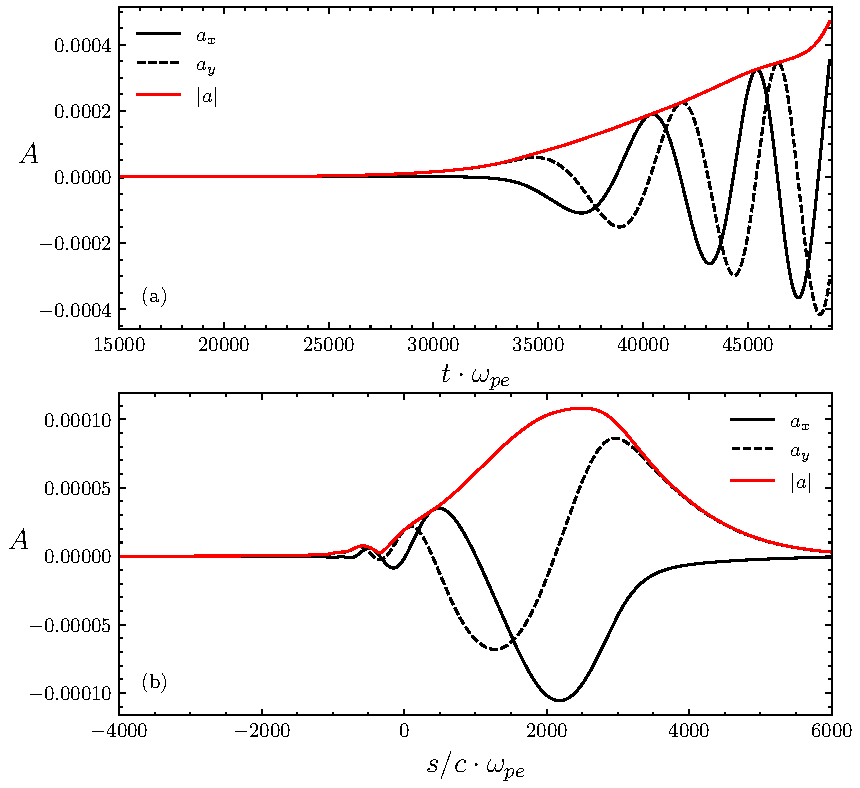
\includegraphics[scale=0.5]{img/aanda.pdf}
    \caption{(a) magnetic field profile and (b) parameter $\Pi$ in our Vlasov simulation. (c) time evolution and (d) spatial distribution of the orthogonal components of vector potential, $a_x$ and $a_y$, and the amplitude $|a|$ in the simulation.
    \label{fig.aanda}
    }
\end{figure}

%In other word, $a$ is a complex number and so does $\omega_b$.

%particle trajectory
The varying phase $\delta \phi(s,t)$ indicates the acceleration of trapped particles along $\Omega$ momentum dimension in phase space.
Combining the calculated wave fields  in the Vlasov simulation \cite{zheng2024}, we solve the equations of motion using the Hamiltonian in Eq. (\ref{eq.H_lab}) and show the particle phase space trajectories in Fig. \ref{fig.phaseflow}(a). 
In the static resonance frame, trapped particles do not have a closed phase space trajectory and  their angle variable $\xi$  is shifting and matching with the wave phase $\delta \phi$ along its trajectory, as illustrated in Fig. \ref{fig.phaseflow}(b). This is in accordance with the phase locking condition \cite{tao_trap-release-amplify_2021}.
Their momenta, as shown in Fig. \ref{fig.phaseflow}(c), are also accelerating upwards along $\Omega$ dimension due to the rising tone frequency chirping.

\begin{figure}
    \centering
    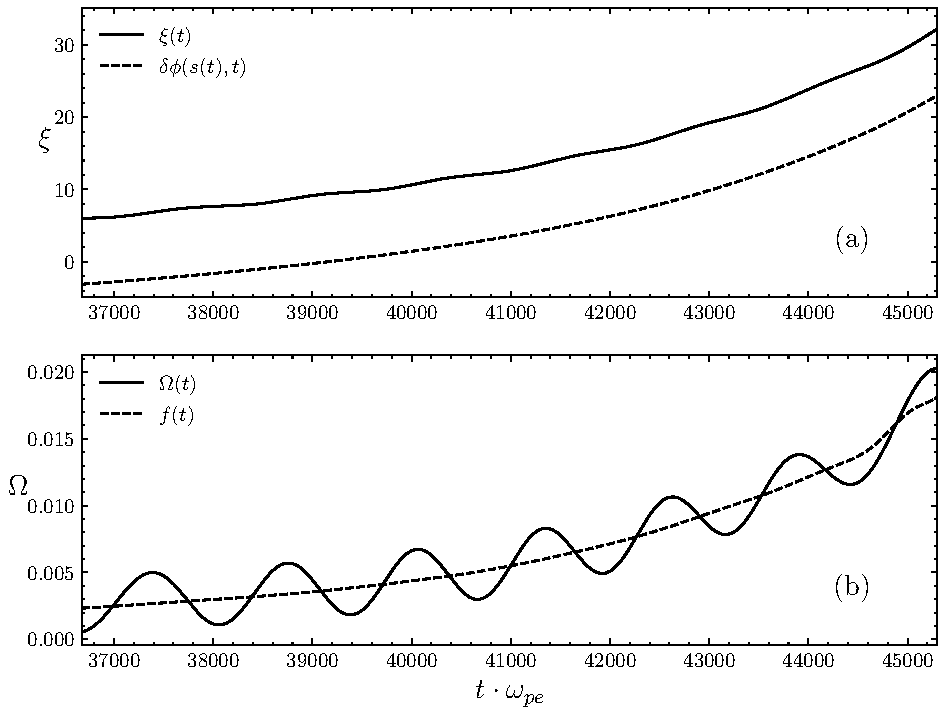
\includegraphics[scale=0.5]{img/phaseflow.pdf}
    \caption{(a) Phase space trajectories of  test particles with initial angle $\xi = 6$ sampled in $\Omega \in [-0.01,0.01]$, (b) typical variation of angle coordinate $\xi$ of a test particle and the corresponding wave phase $\delta \phi$ along its trajectory. (c) the corresponding variation of particle momentum $\Omega$ with time. The dashed line denotes Eq. (\ref{eq.ft}).
    \label{fig.phaseflow}
    }
\end{figure}

Since the wave phase $\delta \phi$ can be calculated from the Vlasov simulation
 \cite{zheng2024}, we can construct a canonical transformation to shift the static resonance frame back to the real-time resonance frame of reference.
To do so, the new angle variable and momentum  take the following forms \cite{berk1999},
\begin{equation}
    \begin{aligned}
        Q &= \xi - \delta \phi(s(t),t)~,
        \\
        P & = \Omega - f(t)~,
    \end{aligned}
\end{equation}
where $f(t)$ is a time dependent function to be determined.
The above transformation corresponds to a type-2 generating function
\begin{equation}
    F_2(\xi,P,t) = (\xi - \delta \phi) \cdot P + \xi \cdot f(t)
\end{equation}
and the corresponding new Hamiltonian $K^\prime$ is
\begin{equation}
    \begin{aligned}
        &  K^\prime = K + \frac{\partial F_2}{\partial t}
        \\
        & = \frac{k_l^2}{2}(P+f(t))^2 
        + \sqrt{2\omega_{ce}(\mathcal{J}+P+f(t)+\Pi)} \cdot |a|\cos(Q) 
        \\
        & + \left(\left(\frac{1}{k_l}(\mathcal{J} - \frac{\Pi}{2} \frac{d\omega_{ce}}{ds}\right)  +\frac{d f(t)}{d t} \right))\cdot(Q + \delta \phi)  - \frac{d \delta \phi}{d t} P ~. 
        \end{aligned}
\end{equation}
In addition,  the first order term with respect to $P$ 
should be eliminated
in the above Hamiltonian, which determines $f(t)$ as
\begin{equation}\label{eq.ft}
    \begin{aligned}
    f(t) & = \frac{1}{k_l^2} \frac{d \delta \phi}{d t}  &= \frac{\delta \omega - v_r \delta k}{k_l^2}~.
    \end{aligned}
\end{equation} 
Note that the exact time derivative is evaluated along the particle trajectory, $d/dt = \partial/\partial t + v_r \partial /\partial s$ with $\delta \omega  \equiv \partial \delta \phi/\partial t$ and $\delta k  \equiv -\partial \delta \phi/\partial s$.
We can examine that $f(t)$ is the first order variation of $\Omega(\omega,k)$ due to the chirping frequency $\delta \omega$, and the variation of wave number $\delta k$.
The expression also agrees with the change of $\Omega$ in the test particle results shown in Fig. \ref{fig.phaseflow}(c).
%\begin{equation}
%    \begin{aligned}
%    \delta \omega & \equiv \frac{\partial \delta \phi}{\partial t}~,
%    \\
%    \delta k & \equiv -\frac{\partial \delta \phi}{\partial s}~,
%    \end{aligned}
%\end{equation}
For the derivative of $f(t)$, we only keep the term up to the first order, which gives
\begin{equation}
    \frac{d f(t)}{d t} \simeq \frac{1}{k_l^2}(\frac{\partial \delta \omega}{\partial t} + 2 v_r \frac{\partial \delta \omega}{\partial s} + \frac{3}{2}v_r\frac{\delta k}{k_l} \frac{d \omega_{ce}}{d s}  ).
\end{equation}
Finally, the new Hamiltonian takes the following form 
\begin{equation}\label{eq.H_frame}
    K^\prime = \frac{k_l^2 P^2}{2} + \frac{{\omega^\prime_{b}}^2}{k_l^2} (\cos Q + \alpha \cdot Q)~,
\end{equation}
where the new bounce frequency $\omega^\prime_{b}$ satisfies
\begin{equation}
    \frac{{\omega^\prime_{b}}^2}{k_l^2} = \sqrt{2\omega_{ce}(\mathcal{J}+P+f(t)+\Pi)}  |a|
\end{equation}
and we have a new $\alpha^\prime$
\begin{equation}\label{eq.alpnew}
    \begin{aligned}
    \frac{{\omega^\prime_{b}}^2}{k_l^2}\alpha^\prime & = \frac{1}{k_l}\left(\mathcal{J} - \frac{\Pi}{2}\right) \frac{d\omega_{ce}}{ds} \\
    & + \frac{1}{k_l^2}\left(\frac{\partial \delta \omega}{\partial t} + 2 v_r \frac{\partial \delta \omega}{\partial s} + \frac{3}{2}v_r\frac{\delta k}{k_l} \frac{d \omega_{ce}}{d s}\right)~.
    \end{aligned}
\end{equation}
The modified parameter now describes the frequency chirping and inhomogeneities in the background magnetic field, and 
the additional terms compared to Eq. (\ref{eq.alpold}) is the first order correction related to frequency chirping and wave number variation.

\begin{figure}
    \centering
    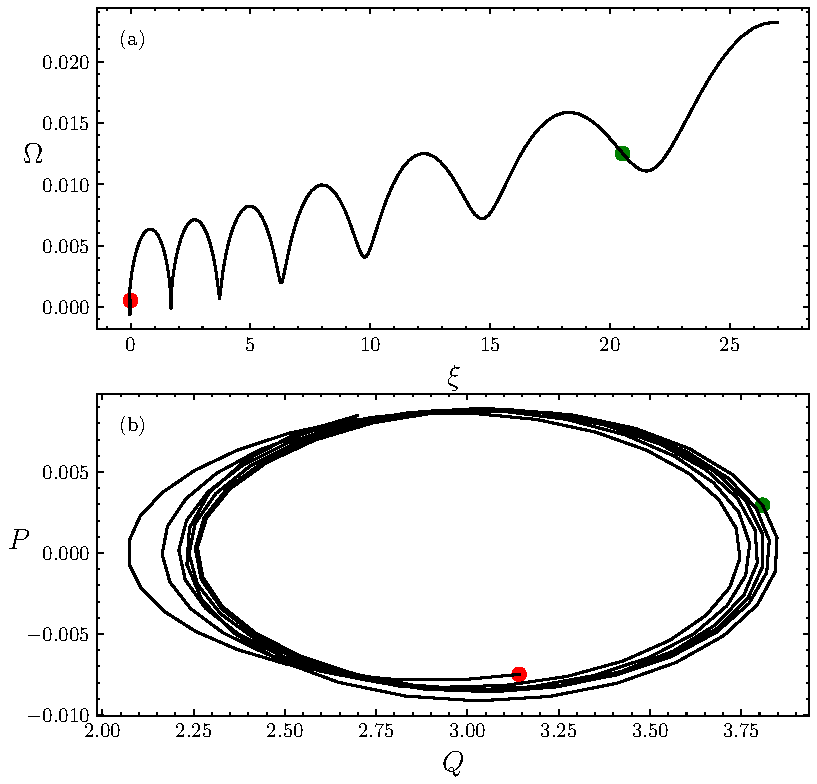
\includegraphics[scale=0.5]{img/Trajectory.pdf}
    \caption{Phase space trajectory of a test particle from $s \simeq 2106.9 c/\omega_{pe}$ at $t\simeq 36675 \omega_{pe}^{-1}$ to $s \simeq 205 c/\omega_{pe}$ at $t=45475.9 \omega_{pe}^{-1}$  in the static resonance frame (a) and  in the real-time resonance frame (b). The red dot denotes the start point, and the green dot denotes $t \simeq 44498  \omega_{pe}^{-1}$ which is the critical point where the adiabatic invariant changes significantly. The corresponding enclosed phase space loop of a particle in static (c) and real-time reference frame (d) at different times.
    \label{fig.traj}
    }
\end{figure}
%Using the wave data from our Vlasov simualtion, we show the contour plot both of the Hamiltonian (\ref{eq.H_lab}) and the modified Hamiltonian (\ref{eq.H_frame}) in Fig. \ref{fig.Hamcontour}. Due to the $\alpha$/$drg$ term in the Hamiltonian, the trapped region is enclosed between a saddle point  and a C point.
With the constructed Hamiltonian, we are able to consider the particle dynamics in real-time resonance frame of reference.
The phase space trajectory is determined from the Hamilton's canonical equation,
\begin{equation}
    \begin{aligned}
        \frac{d\Omega}{dt} &= - \sqrt{2\omega_{ce}(s)\mu(s)} \mathbb{I} (a(s,t)\cdot e^{-\imath \xi}) - \frac{\omega^2_{b}}{k_l^2(s)} \alpha
        \\
        \frac{d\xi}{dt} &= k_l^2(s) \Omega +\sqrt{\frac{\omega_{ce}(s)}{2\mu(s)}} \mathbb{R}(a(s,t)\cdot e^{-\imath \xi})
    \end{aligned}
\end{equation}
where $\mu(s) = \mathcal{J}(s)+\Pi(s)+\Omega$ is the magnetic moment.
For $Q-P$ space, the equation is similar with only substitution of the parameter to new $\alpha^\prime$ and ${\omega^\prime_{b}}^2$.

For both Hamiltonian, we choose a test particle initially locate at $s \simeq 2106.9 c/\omega_{pe}$ at $t\simeq 36675 \omega_{pe}^{-1}$. We show the corresponding Hamiltonian at this location in Fig. \ref{fig.Hamcontour}. We set the particle to been initially trapped at the resonance center, and calculate its phase space trajectories, the result is shown in Fig. \ref{fig.traj}. At each $s$ location, we push the phase flow from current time $t$ to $t+\Delta T$ where $\Delta T= 48.9 \omega_{pe}^{-1}$ using time-adaptive Runge-Kutta method, then we push the resonant particle along the field line according to their characteristic lines in $s$ $\mathcal{J}$ space.
The procedure is in accordance with our Euler-Lagrangian hybrid Vlasov method.
%It can be found that 
In the static  resonance frame, the particle suffers a rapid change in $\Omega$ for each bounce in accordance with  Fig. \ref{fig.phaseflow}(a).
In contrast, there exists only a slight change when we track the particle in the real-time resonance frame, which demonstrates the effectiveness of the canonical transformation.


